\section{Modelo de Ising}


El Hamiltoniano del modelo de Ising transversal es
\begin{equation*}
    H=-\omega\qty(\sum_{\langle j,k \rangle}\pauli{3,j}\otimes\pauli{3,k}+g\sum_{k}\Id\otimes\pauli{1,k}),
\end{equation*}

que, si $g=0$ (fase ordenada) y tomando en cuenta únicamente un par de partículas se convierte en el Hamiltoniano de interacción
\begin{equation*}
    H=-\omega \pauli{3}\otimes\pauli{3}.
\end{equation*}

Dado un estado efectivo $\rho\in\densityspace{2}$, propagar al estado asignando a través del Principio de Máxima Entropía con dicha evolución y luego tomar la descripción dada por la aplicación de grano grueso resulta en la dinámica efectiva
\begin{align*}
    \Gamma_{t}^{p}(\rho)=&\rho \cos^{2}(\omega)+\pauli{3} \rho \pauli{3} \sin^{2}(\omega t)\\
    & + i\sin(\omega t)\cos(\omega t)\qty(p\expval{\pauli{3}}_{B}[\pauli{3},\rho_{A}]+(1-p)\expval{\pauli{3}}_{A}[\pauli{3},\rho_{B}]).
\end{align*}
Reconocemos dos términos: uno lineal y uno no lineal. El primero tiene forma de canal de desfasamiento sobre el estado efectivo. El segundo depende de los parámetros de la aplicación de grano grueso y de los valores esperados con respecto a los operadores de densidad reducidos del estado de máxima entropía. En efecto, el caso límite $p=1$ o $p=1$ simplemente reduce la dinámica a un canal de desfasamiento:

\begin{equation*}
    \Gamma_{t}^{p=1}(\rho)=\rho \cos^{2}(\omega)+\pauli{3} \rho \pauli{3} \sin^{2}(\omega t).
\end{equation*}

mientras que el caso $p=\frac{1}{2}$ revela el efecto del término no lineal:

\begin{equation*}
    \Gamma_{t}^{p=\frac{1}{2}}(\rho)=\rho \cos^{2}(\omega)+\pauli{3} \rho \pauli{3} \sin^{2}(\omega t) + i\expval{\pauli{3}} \qty[\pauli{3},\rho] \sin(\omega t)\cos(\omega t).
\end{equation*}

Nótese que, si del factor $\expval{\pauli{3}}=1$, la dinámica sería no solo lineal, sino unitaria, y correspondería a una rotación respecto al eje $z$, de no ser que los únicos estados tales que $\expval{\pauli{3}}=1$ son invariantes bajo dichas rotaciones. En realidad, lo que se observa es que la dinámica efectiva es una rotación respecto a $z$ que depende de la componente en $z$ del estado efectivo inicial. Cuando $\expval{\pauli{3}}=0$, la dinámica es un canal de despolarización que manda a todos los estados al eje $z$ (a un tiempo $\omega t =\frac{\pi}{4}$). 

\begin{figure}[ht!]
    \centering
    \begin{subfigure}{0.32\textwidth}
      \centering
      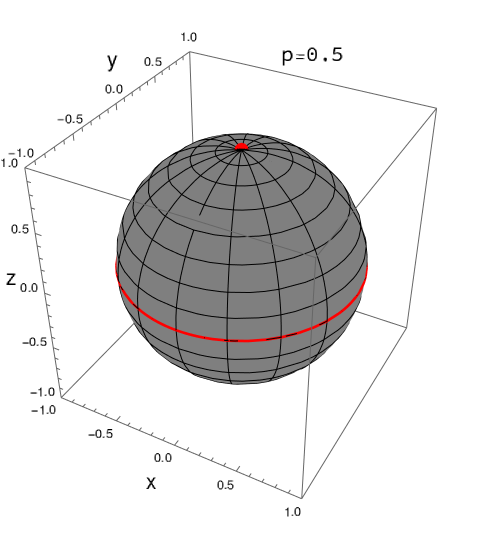
\includegraphics[width=0.9\linewidth]{../thesis/chapter3/figures_special/sphere_Ising_t=0._z=0.9_p=0.5.png}
      \caption{$t=0$}
    \end{subfigure}%
    \begin{subfigure}{0.32\textwidth}
      \centering
      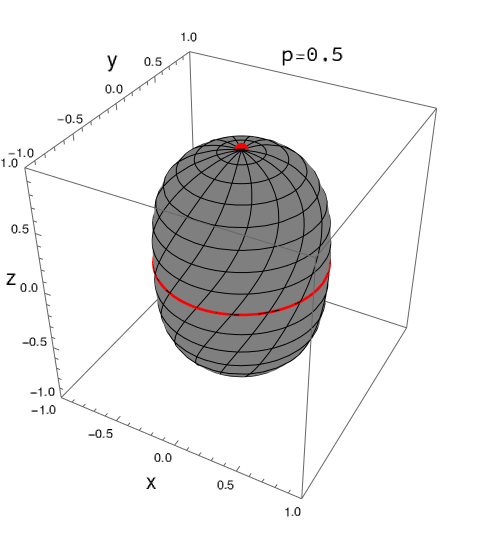
\includegraphics[width=0.9\linewidth]{../thesis/chapter3/figures_special/sphere_Ising_t=0.5_z=0.9_p=0.5.png}
      \caption{$t=0.5$}
    \end{subfigure}
    \begin{subfigure}{0.32\textwidth}
      \centering
      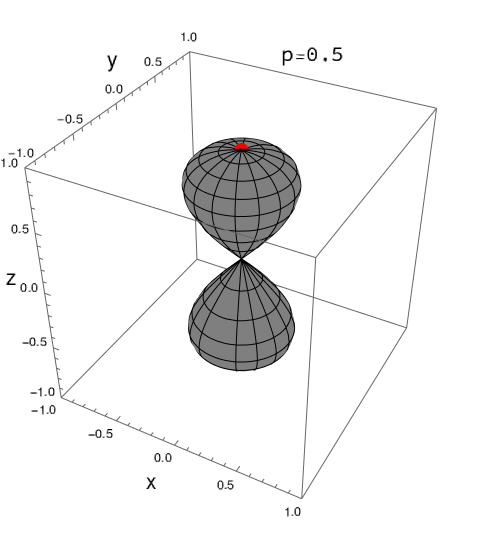
\includegraphics[width=0.9\linewidth]{../thesis/chapter3/figures_special/sphere_Ising_t=1._z=0.9_p=0.5.png}
      \caption{$t=1$}
    \end{subfigure}
    \caption{Efecto del la evolución sobre la esfera de Bloch cuando $p=\frac{1}{2}$. Nótese que el desfasamiento sólo se completa en el eje $xy$.}
    \label{fig:Ising_p0.5_Sequence}
    \end{figure}

La despolarización dependiente de la componente en $z$ inicial es más clara si se observa el efecto de la evolución sobre el vector de Bloch. Abusando un poco de la notación se nota que 

\begin{equation*}
    \Gamma_{t}^{p=\frac{1}{2}}(\vec{r}_{\rho})=\begin{pmatrix}
        x\cos(2\omega t)-yz\sin(2\omega t)\\
        y\cos(2\omega t)+xz(2\omega t)\\
        z\\
    \end{pmatrix}
\end{equation*}
\acnote{Aquí se ve la casi rotación, pero creo que lo tengo que descomponer en diferentes operaciones para notar que el desfasamiento se da de forma más fuerte conforme más pequeño es z}